\section{\label{sec:SoA}Introduction}
Developing products, especially lightweight structures, 
requires variety of steps to come from the original idea to the final product.
One approach to follow these steps to result in a successful production 
are described in the guidelines of VDI 2206 \cite{gausmeier2002} and VDI 2221 \cite{Jansch2006THEDO}.
These guidelines give a general methodology for designing technical systems and products, 
by introducing a methodical and systematic designing procedure, to work with maximum efficiency.
Since the first introduction in 1993 these guidelines have been applied within mechanical engineering, precision mechanics, 
switches and software development and the planning of process engineering \cite{pahl_beitz_2013}. 
Depending on the individual outcome steps might be repeated in as part of cyclic quality enforcing technique.
Especially in lightweight design the analysis, design and manufacturing processes are so strong connected, 
that they all have to be considered in every phase of the development process (fig. \ref{pic:interactive-design}).
The amount of cyclic repeats do increase with higher demands on the products efficiency and error margin.
These causes it to be one of the main factors for increased development time and 
also reduces the amount of reusable components with slightly changes in the product demand.\\
\begin{figure}[h]
    \centering
    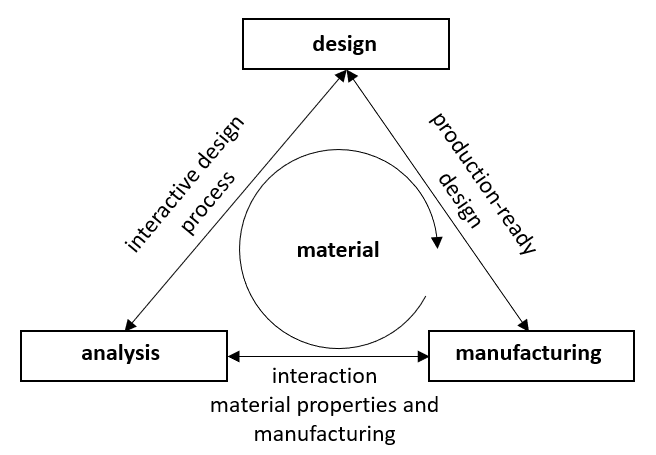
\includegraphics[scale=0.5]{pics/interactive-design.PNG}
    \caption{\label{pic:interactive-design} "A spiral development approach for complex function‐integrative systems." \cite{bohm_interaktiver_2020}}
\end{figure}\\
Further, with increasing complexity the number of required experts increases.
This often can lead to miss-communication between the experts themselves or in translation problems 
to transfer information form one system to another (CAD-chains).\\
Using the advantages of digital technologies is since the dawn of computer aided design (CAD) in the mid-1960s
a lot of research has been done to solve these issues. 
Resulting in row of CAD-systems, Simulation programs and product data management (PDM) systems.
But especially notable was E. Allen, who showed in 1970, that these kind of systems, 
can be described as a directed graph, consisting of a set of nodes and directed edges, 
which are connecting the nodes with each other \cite{allen_control_1970}.
Each node hereby describes a linear sequence of program instructions, 
what means that nodes have one entry point (the first instruction executed) and 
one exit point (the last instruction executed).
Following along the edges, in a directed graph, results in a series of blocks what is called a path.
This description allows to also describe closed path or circuit is a paths, 
where the path ends at the same start block. 
\cite{allen_control_1970}\\
Problems that can be described with these models are summarized 
under the term 'directed graph theory' \cite{bang-jensen_digraphs_2009, lehman_directed_2010}
and have been studied for a wide variety of different applications in 
\cite{lehman_directed_2010, aho_theory_1972, kam_global_1976}.\\
Graph based solutions are often characterized as easy to understand and to compute, 
but also have difficulties if the causality can change dynamically \cite{sinha_modeling_2001}. 
Further, with systems like CAMP-G and SIDOPS+ \cite{breunese_modeling_1996} mechanism to solve 
nonlinear high-dimensional graph models that can contain both continuous-time and 
discrete-time parts have been developed.\\
Today, Graph-Based Approaches has been implemented in a handful of design programs and 
simulations tools \cite{noauthor_dynamo_2020, noauthor_function_2020, noauthor_systems_2020},
but none of these implementations allows the use of processes of other design or simulation tools.\\
Complex multi-disciplinary systems requires the expertise of a group of collaborating specialists:
Designers with backgrounds in different disciplines collaborate with analysts, manufacturing engineers, marketing
specialists, and business managers.\cite{sinha_modeling_2001}\\
Therefor computer aided engineering (CAE) technologies, that provide sharing, visualization, 
documentation, and management of product models,
are used to coordinate design processes among geographically dispersed and multidisciplinary
teams \cite{finger_creating_1994, bajaj_web_1999, iwasaki_web-based_2002}.
However, the aspect of collaborative simulation modeling is still in its infancy. 
The current approach to support collaborative modeling, is done by shared model representations, 
repositories to manage model components, and model abstraction capabilities to provide different views of models to designers.
Therefore designers need a common model representation to share simulation models within a collaborative modeling environment.\cite{sinha_modeling_2001}\\
This approach has been used in the development of the Very High-Speed Integrated Circuit Hardware Description Language (VHDL),
which has been used as a design automation tool in all phases of modern very large-scale integration (VLSI) design. 
Similarly, the U.S. Department of Defense and its contractors have used the High Level Architecture (HLA) for simulation of
battlefield scenarios \cite{lutz_high_1998,park_relational_1994}.
Future modeling and simulation environments should allow for a tight integration
between application domains, either by interfacing the solvers or by using common model representations.
To further improve the exchange of model information, researchers have started to develop domain ontologies \cite{devedzic_survey_1999}. 
\cite{ozawa_model_2000} proposed a common ontology to support different levels of information sharing between humans and multiple
modeling and simulation software agents. 
Upon these domain ontologies, unified taxonomies and keyword networks
can be built to support model retrieval and repository management.\\
If a complex multi-disciplinary systems can be modelled sufficiently, the question of the optimal solution rises.
A big issue that the system behavior, id hard to predict.
Therefore only optimizations approaches will be discussed, which can deal with systems,
where the system can be considered as a black box, excluding approaches like Gradient descent method.
Further it is important to make sure to find the global optimum and not to fall in local minima.
Therefor suitable approaches are: simulated annealing \cite{khachaturyan_thermodynamic_1981}, 
evolutionary algorithm \cite{wu_ensemble_2019}, particle swarm optimization \cite{Kennedy1995} and Bayesian optimization \cite{marcuk_optimization_1975}.\\
In \cite{hornby_automated_2006, khalafallah_electimize_2011, evans_aerodynamic_2017, slagter_perform_2020}
single domain based simulations have been combined with optimization methods.\\
However, the question remains, if a system can be designed to sufficiently describes the  
the causalities of a complex multi-disciplinary systems and if so, 
could it be used to optimize a complex product.